\begin{figure}[htbp]
\centering
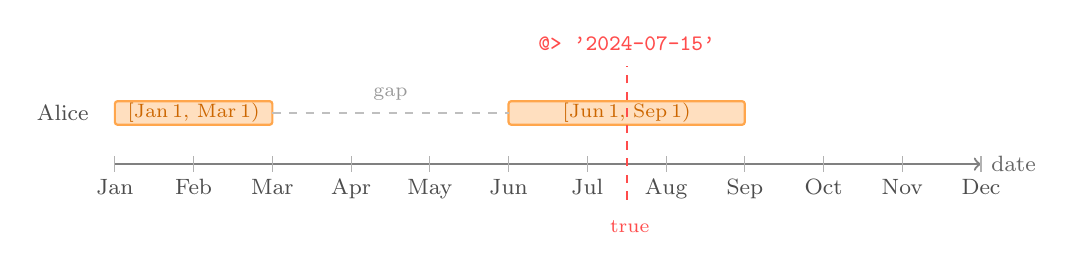
\begin{tikzpicture}[
  font=\small,
  axis/.style={->, black!50, thick},
  bar/.style={draw=none, rounded corners=1pt, minimum height=9pt},
  label/.style={font=\footnotesize, black!70},
]

%% ── timeline axis ──────────────────────────────────────────────────
\def\TL{11.0}   % total axis length (cm)
\draw[axis] (0,0) -- (\TL,0) node[right, font=\footnotesize, black!60] {date};

%% month tick marks and labels (Jan=0 … Dec=11, spaced 1 cm apart)
\foreach \mo/\lbl in {
  0/Jan, 1/Feb, 2/Mar, 3/Apr, 4/May, 5/Jun,
  6/Jul, 7/Aug, 8/Sep, 9/Oct, 10/Nov, 11/Dec}
{
  \draw[black!30] (\mo, 0.10) -- (\mo,-0.10);
  \node[label, below=2pt] at (\mo,0) {\lbl};
}

%% ── Alice's two availability windows ──────────────────────────────
\def\barY{0.65}
\node[label, left=6pt] at (0, \barY) {Alice};

%  window 1: [Jan 1, Mar 1)  →  x=0 .. x=2
\fill[orange!25, rounded corners=1pt]
  (0, \barY-0.15) rectangle (2, \barY+0.15);
\draw[orange!70, thick, rounded corners=1pt]
  (0, \barY-0.15) rectangle (2, \barY+0.15);
\node[font=\scriptsize, orange!80!black] at (1, \barY)
  {[Jan\,1, Mar\,1)};

%  window 2: [Jun 1, Sep 1)  →  x=5 .. x=8
\fill[orange!25, rounded corners=1pt]
  (5, \barY-0.15) rectangle (8, \barY+0.15);
\draw[orange!70, thick, rounded corners=1pt]
  (5, \barY-0.15) rectangle (8, \barY+0.15);
\node[font=\scriptsize, orange!80!black] at (6.5, \barY)
  {[Jun\,1, Sep\,1)};

%% ── @> query: vertical dashed line at Jul 15 (x ≈ 6.5) ──────────
\def\QX{6.5}
\draw[red!70, dashed, thick] (\QX, -0.45) -- (\QX, 1.25);
\node[red!70, font=\footnotesize, above=2pt] at (\QX, 1.25)
  {\texttt{@> '2024-07-15'}};
\node[red!70, font=\scriptsize, below=4pt] at (\QX, -0.45)
  {$\checkmark$\;true};

%% ── gap annotation ────────────────────────────────────────────────
\draw[black!25, dashed] (2, \barY) -- (5, \barY);
\node[font=\scriptsize, black!40, above=1pt] at (3.5, \barY) {gap};

\end{tikzpicture}
\caption{A \texttt{datemultirange} with two sub-ranges; \texttt{@>} checks containment across all.}
\label{fig:multirangecontains}
\end{figure}
